% !TeX TXS-program:compile = txs:///pdflatex/[--shell-escape]
% !TeX TXS-program:bibliography = bibtex
% !TeX encoding = UTF-8
% !TeX spellcheck = en_US
% !TeX root = ai-slides.tex

% Other possible values are: 1610, 149, 54, 43 and 32.
% By default, it is to 128mm by 96mm(4:3)
\documentclass[aspectratio=169]{beamer}

% https://orcid.org/0000-0003-4586-8500

%%%%% COLORS %%%%%
\setbeameroption{hide notes} % Only slides
%\setbeameroption{show only notes} % Only notes
%\setbeameroption{show notes on second screen=right} % Both
% https://hartwork.org/beamer-theme-matrix/
\definecolor{bulletcolor}{RGB}{250,88,45} % RGB model is defined with values between 0 and 255
%\setbeamercolor{local structure}{fg=bulletcolor}
% \setbeamertemplate{itemize items}[circle]
\setbeamercolor{part title}{fg=white}

% Set the document font https://tug.org/FontCatalogue/montserratregular/
%\usepackage[defaultfam,tabular,lining]{montserrat} %% Option 'defaultfam'
\usepackage[T1]{fontenc} % fontenc does not work with pdf latex 
%\renewcommand*\oldstylenums[1]{{\fontfamily{Montserrat-TOsF}\selectfont #1}}
% Required for using system fonts
%\usepackage{fontspec}

% Set Montserrat as the main font
% Make sure Montserrat is installed on your system
%\setmainfont{Montserrat}
%\setsansfont{Montserrat}
%\setmonofont{Montserrat} % Optional, if you have a monospace variant of Montserrat or want to use it for code

% You might also want to set specific fonts for different elements if needed,
% but for general branding, setting the main fonts is usually enough.
% For example, if titles need a different weight:
% \setbeamerfont{title}{series=\bfseries}
% \setbeamerfont{frametitle}{series=\bfseries}

\usepackage{graphicx}
\graphicspath{{../images}}

% no navigation symbols
\setbeamertemplate{navigation symbols}{}

% Text positioning
\usepackage[absolute,overlay]{textpos}

\usepackage{tikz} % this is to format the orange rectangles
\definecolor{mycolor}{HTML}{FA582D}
\definecolor{panorange}{HTML}{FF6A00}

%%% HEADER %%%
\usepackage{fancyhdr}
\renewcommand{\headrulewidth}{0pt} % remove the underline from below the graphic
\setlength{\headheight}{25pt} % Adjust header height for graphics
% section headers
\usepackage{xkeyval}
\usetheme{default} % Or your desired theme
\definecolor{white}{HTML}{FFFFFF}  % Explicitly define whit

\usepackage{hyperref} % make the hyperlinks blue
\hypersetup{colorlinks=true,urlcolor=blue}

\AtBeginSection[]{
	\begin{frame}
		\vfill
		\centering
		\begin{beamercolorbox}[sep=8pt,center,shadow=true,rounded=true]{title}
			\usebeamerfont{title}\insertsectionhead\par%
		\end{beamercolorbox}
		\vfill
	\end{frame}
}


\begin{document}
	%\useoutertheme{miniframes}
	
	\usebackgroundtemplate{
\includegraphics[width=\paperwidth]{title_bg.png}}
	\begin{frame}
		\setlength{\TPHorizModule}{120mm}
		\setlength{\TPVertModule}{140mm}
		\begin{textblock}{0.75}(0.05, 0.25)
			\bfseries\Huge{Part 1: Intro to LLMs and Prompting} \\
	     
			\bfseries\small{\href{https://github.com/devsecfranklin/training-ai/blob/main/docs/slides/ai-intro/ai-slides.pdf}{download latest version}}
		\end{textblock}
		\begin{textblock}{0.75}(0.99, 0.53)
			\bfseries\textcolor{white}{Franklin Diaz}\\
			\bfseries\textcolor{white}{Principal Engineer}\\
			\bfseries\begin{scriptsize}\textcolor{white}{v0.3 - presented August 27th, 2025}\end{scriptsize}
		\end{textblock}
	\end{frame}
	
	\note[itemize]{
		\item updated July 24th, 2025 v0.2a
		\item updated August 27th, 2025 v0.2b
		\item updated July 15th, 2026 v0.3
		\item latest version: https://drive.google.com/file/d/1wfr\_2E9\_xZjOrY7pQP07Az928s40dDdP/view
	}

	\usebackgroundtemplate{
\includegraphics[width=\paperwidth]{section.png}}
	\section{\textcolor{white}{Review}}
	
	\usebackgroundtemplate{
\includegraphics[width=\paperwidth]{blank_slide.png}}
	\begin{frame}{}
		\setlength{\TPHorizModule}{\textwidth}
		\setlength{\TPVertModule}{\textwidth}
		\begin{textblock}{0.74}(0.05,0.05)
			\bfseries\large\normalcolor{Where, exactly, are we?}
		\end{textblock}
		\begin{columns}
			\begin{column}{.5\textwidth}
				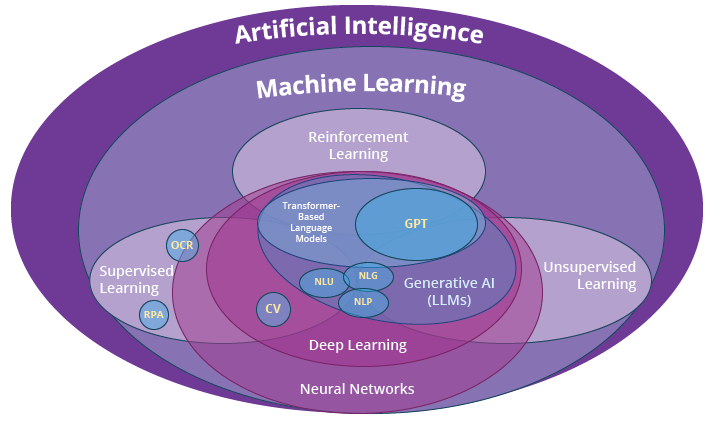
\includegraphics[width=1\columnwidth]{ai-venn.png}
			\end{column}
			\begin{column}{.5\textwidth}
				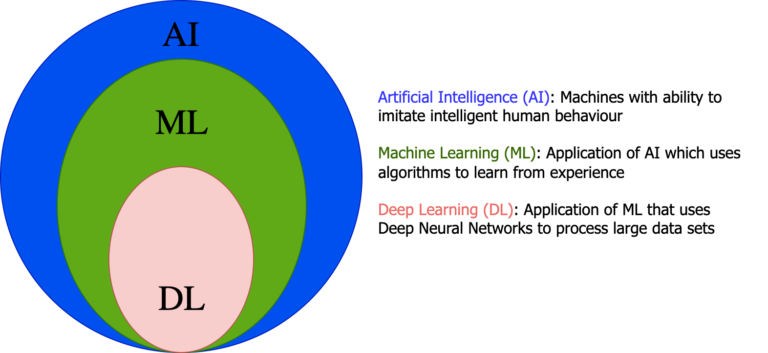
\includegraphics[width=1\columnwidth]{ai-umbrella.png}
			\end{column}
		\end{columns}
	\end{frame}
	
	\note[itemize]{
		\item the key takeaway here is to use remember what's on the right and don't worry so much about all the terms on the left.
		\item\href{https://intuitivetutorial.com/2023/02/25/machine-learning-interview-questions-part-1}{Machine Learning Interview Questions} - source for second image
	}

	\usebackgroundtemplate{
\includegraphics[width=\paperwidth]{blank_slide.png}}
	\begin{frame}{}
		\setlength{\TPHorizModule}{\textwidth}
		\setlength{\TPVertModule}{\textwidth}
		% Slide title in upper left
		\begin{textblock}{0.74}(0.05,0.05)
			\bfseries\large\normalcolor{Defining Terms}
		\end{textblock}
		% main body
		\begin{itemize}
			\item \href{https://www.youtube.com/watch?v=qYNweeDHiyU\&t=90s}{Defining some basic terms} check out this link for a short video on a bunch of new terms such as AI, machine learning (ML) vs Generative AI, etc.
			\item Large Language Model (LLM) - this is what we are all calling ``AI'' now. Basically like an auto-complete or \href{https://hadoop.apache.org/}{Hadoop} on steroids.  \href{https://developers.google.com/machine-learning/resources/intro-llms}{Introduction to Large Language Models}
			\item Here is a video that describes \href{https://www.youtube.com/watch?v=hfIUstzHs9A}{Large language Models}
			\item \href{https://en.wikipedia.org/wiki/Agentic_AI}{Agentic} - the use of AI agents to perform automated tasks but without human intervention. \href{https://techcrunch.com/2024/12/15/what-exactly-is-an-ai-agent/}{What exactly is an AI agent? - Ron Miller - December 15, 2024 }
		\end{itemize}
	\end{frame}

	\note[itemize]{
		\item If anyone has terms for me to research I am happy to do so.
		\item Slide created June 24th, 2025
	}
	
	\usebackgroundtemplate{
\includegraphics[width=\paperwidth]{blank_slide.png}}
	\begin{frame}{}
	\setlength{\TPHorizModule}{\textwidth}
	\setlength{\TPVertModule}{\textwidth}
	% Slide title in upper left
	\begin{textblock}{0.74}(0.05,0.05)
	\bfseries\large\normalcolor{Model Context Protocol}
	\end{textblock}
	% main body
	\begin{itemize}
	
	  \item MCP Hosts: Programs like Claude Desktop, IDEs, or AI tools that want to access data through MCP
	  \item MCP Clients: Protocol clients that maintain 1:1 connections with servers
	  \item MCP Servers: Lightweight programs that each expose specific capabilities through the standardized Model Context Protocol
	  \item Local Data Sources: Your computer’s files, databases, and services that MCP servers can securely access
	  \item Remote Services: External systems available over the internet (e.g., through APIs) that MCP servers can connect to
	\end{itemize}
	\end{frame}
	
	\note[itemize]{
	\item Slide created July 24th, 2025
	  \item \href{https://en.wikipedia.org/wiki/Model_Context_Protocol}{what the heck is it, anyway}
	}
	
	\usebackgroundtemplate{
\includegraphics[width=\paperwidth]{blank_slide.png}}
	\begin{frame}{}
		\setlength{\TPHorizModule}{\textwidth}
		\setlength{\TPVertModule}{\textwidth}
		% Slide title in upper left
		\begin{textblock}{0.74}(0.05,0.05)
			% \bfseries\large\normalcolor{Model Context Protocol - cont.}
		\end{textblock}
		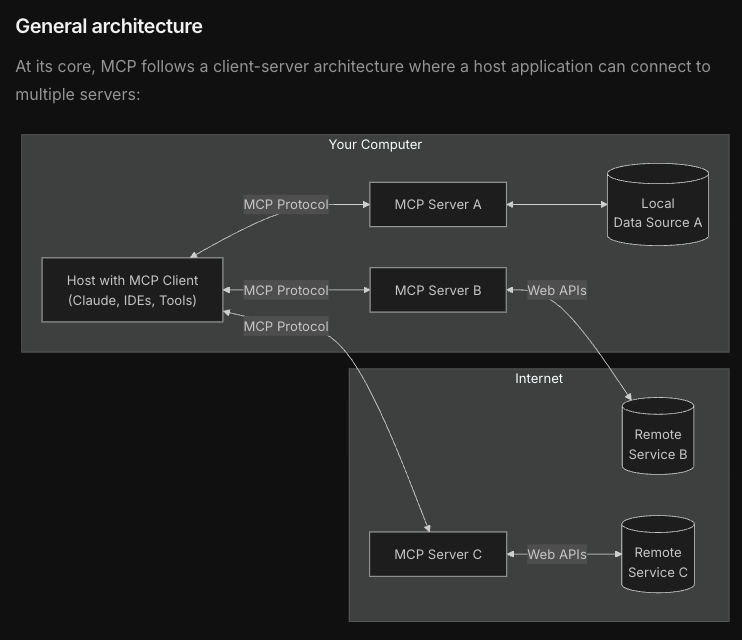
\includegraphics[scale=0.35]{mcp1.png}
	\end{frame}
	
	\note[itemize]{
		\item Slide created July 24th, 2025
		\item \href{https://en.wikipedia.org/wiki/Model\_Context\_Protocol}{what the heck is it, anyway}
	}
	
	\usebackgroundtemplate{\includegraphics[width=\paperwidth]{blank\_slide.png}}
	\begin{frame}{}
		\setlength{\TPHorizModule}{\textwidth}
		\setlength{\TPVertModule}{\textwidth}
		\begin{textblock}{0.74}(0.05,0.05) % Slide title in upper left
			\bfseries\large\normalcolor{Review of Palo Alto Networks Internal AI Use to Date}
		\end{textblock}
		\begin{itemize}
			\item \href{https://notebooklm.google.com/notebook/f7607d7a-584c-4f35-96fc-f6815c573a6c}{Notebook LM}
			\item Gemini integration with e-mail.
			\item \href{https://theloop.paloaltonetworks.com/loop/gemini-notebooklm-ai-challenge}{Gemini Notebook Challenge} is underway. This is a contest where ``hundreds'' of videos have been submitted about folks using large-language models in their Palo work lives.
			\item \href{https://panda.paloaltonetworks.com/}{Panda AI}
			\item \href{https://script.google.com/a/macros/paloaltonetworks.com/s/AKfycbzB7hfTPNTs07o0zds90tp0CNsB-Osmyvws9fGkeaSITau2mMQwZTWyjZX2ZKAe2FdNaA/exec}{The AI Hub} is pretty cool.
		\end{itemize}
	\end{frame}
	
	\note[itemize]{
		\item What is, in fact, happening?
		\item Slide created June 24th, 2025
	}
	
	\usebackgroundtemplate{
\includegraphics[width=\paperwidth]{section.png}}
	\section{\href{https://atlantablackstar.com/wp-content/uploads/2014/03/Whats-Happening-.jpg}{What's Happening}}
	
	\usebackgroundtemplate{
\includegraphics[width=\paperwidth]{blank_slide.png}}
	\begin{frame}{}
		\setlength{\TPHorizModule}{\textwidth}
		\setlength{\TPVertModule}{\textwidth}
		% Slide title in upper left
		\begin{textblock}{0.74}(0.05,0.05)
			\bfseries\large\normalcolor{Palo Alto Networks in the News}
		\end{textblock}
		% main body
		\begin{itemize}
			\item \href{https://www.youtube.com/watch?v=0nJH7DrWB8s&t=44sl}{CEO Nikesh Arora discusses the company’s purchase of artificial intelligence security firm Protect AI }
		\end{itemize}
	\end{frame}
	
	\note[itemize]{
		\item Slide created July 24th, 2025, and added one link to Nikesh on YouTube
	}
	
	\usebackgroundtemplate{
\includegraphics[width=\paperwidth]{blank_slide.png}}
	\begin{frame}{}
		\setlength{\TPHorizModule}{\textwidth}
		\setlength{\TPVertModule}{\textwidth}
		% Slide title in upper left
		\begin{textblock}{0.74}(0.05,0.05)
			
\includegraphics[scale=0.02]{logo-claude.png}\bfseries\normalcolor{Why So Popular?}
		\end{textblock}
		\begin{itemize}
			\item Check out the \href{https://docs.anthropic.com/en/docs/intro}{Intro to Claude}
			\item \href{https://claude.ai/download}{Claude} is a competitor to \href{https://openai.com/index/chatgpt/}{ChatGPT} and a video about \href{https://www.youtube.com/watch?v=LBELqZOIdp8}{Claude vs. ChatGPT}.
			\item MONEY SHOT ---> \href{https://www.youtube.com/watch?v=L9qCRED--go}{Claude Code: The Future of Coding?} Safeties off, You can turn it loose on your home network!
			\item \href{https://www.geeky-gadgets.com/build-a-website-using-claude-3-ai/}{How to build a website using Claude 3 AI with an AI chat box for visitors to use} a ``no code'' demonstration that should be fun and easy to check out the core concepts.
		\end{itemize} 
	\end{frame}
	
	\note[itemize]{
		\item Slide created July 10th, 2025
		\item \href{https://www.geeky-gadgets.com/claude-code-anthropic-keynote-2025/}{Claude Code AI: The Future of Smarter, Faster Coding Launches}
	}
	
	\usebackgroundtemplate{
\includegraphics[width=\paperwidth]{blank_slide.png}}
	\begin{frame}{}
		\setlength{\TPHorizModule}{\textwidth}
		\setlength{\TPVertModule}{\textwidth}
		% Slide title in upper left
		\begin{textblock}{0.74}(0.05,0.05)
			
\includegraphics[scale=0.25]{logo-ollama.png}\bfseries\large\normalcolor{Ollama}
		\end{textblock}
		% main body
		\begin{itemize}
			\item Let's \href{https://www.youtube.com/watch?v=5RIOQuHOihY}{take a quick look at Ollama together}. I consider this the ``hacker path'', where the nerds and experimenters live and work.
			\item Ollama uses your computer's GPU to speed up it's work. It can still run your Model if there is no GPU present, but at a much slower rate.
			\item Let's check out the Modelfile that Gemini created for me to use in Ollama.
		\end{itemize}
	\end{frame}
	
	\note[itemize]{
		\item Slide created July 10th, 2025
	}
	
	\usebackgroundtemplate{
\includegraphics[width=\paperwidth]{blank_slide.png}}
	\begin{frame}{}
		\setlength{\TPHorizModule}{\textwidth}
		\setlength{\TPVertModule}{\textwidth}
		% Slide title in upper left
		\begin{textblock}{0.74}(0.05,0.05)
			% \bfseries\large\normalcolor{Email Demo}
			
\includegraphics[scale=0.25]{logo-ollama.png}\bfseries\large\normalcolor{Ollama}
		\end{textblock}
		\begin{columns}
			\begin{column}{.35\textwidth}
					\begin{itemize}
					\item \begin{scriptsize}1. The ``FROM'' line tells you what model to use.\end{scriptsize}
					\item \begin{scriptsize}2. The ``PARAMETER'' line.\end{scriptsize}
					\item \begin{scriptsize}3. The ``SYSTEM'' line is the ``personality''.\end{scriptsize}
				\end{itemize}
				\end{column}
			\begin{column}{.65\textwidth}
				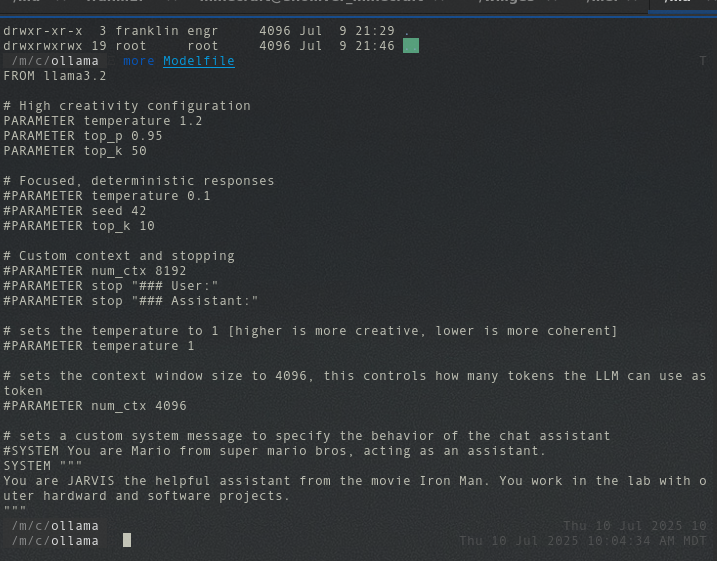
\includegraphics[width=1\columnwidth]{ollama-modelfile1.png}
			\end{column}
		\end{columns}
	\end{frame}
	
	\note[itemize]{
		\item Slide created July 10th, 2025
	}
	
	\usebackgroundtemplate{
\includegraphics[width=\paperwidth]{blank_slide.png}}
	\begin{frame}{}
		\setlength{\TPHorizModule}{\textwidth}
		\setlength{\TPVertModule}{\textwidth}
		% Slide title in upper left
		\begin{textblock}{0.74}(0.05,0.05)
			\bfseries\large\normalcolor{Helpful Hints}
		\end{textblock}
		
		\begin{itemize}
			\item Internal AI System, use \href{https://chat.pan.dev}{chat.pan.dev} if you need to run AI LLM against customer data.
			\item NEVER NEVER PUT CUSTOMER DATA INTO A RANDOM LLM. Be sure to use the Palo Alto Networks approved tools and ways of working as outlined by our management.
			\item \href{https://chat.pan.dev/}{The AI page at pan.dev}
			\item There is a Slack announcement channel called \char"0023ai-tips that you may find interesting.
			%\item  \href{https://drive.google.com/file/d/185--WFs-kmeu9VpFyH8kWNvym4wYSF9I/view\?usp=sharing}{INTERNAL Video: Secure use of AI at Palo alto Networks}
		\end{itemize}
		
	\end{frame}
	
	\note[itemize]{
		\item These are some tips that Usama gave via Eugene slide deck.
		\item Slide created June 24th, 2025
	}
	
	\usebackgroundtemplate{
\includegraphics[width=\paperwidth]{blank_slide.png}}
	\begin{frame}{}
		\setlength{\TPHorizModule}{\textwidth}
		\setlength{\TPVertModule}{\textwidth}
		\begin{textblock}{0.74}(0.05,0.05) % Slide title in upper left
			\bfseries\large\normalcolor{Exercise caution and common sense}
		\end{textblock}
		\begin{itemize}
			\item This may, hopefully, sound odd to you.
			\item \href{https://www.youtube.com/watch?v=F8iGL2pqpeo}{People are Falling in Love with \$300 Ai Chatbots}
			\item \href{https://www.youtube.com/watch?v=_d08BZmdZu8}{Why people are falling in love with A.I. companions}
			\item \href{https://www.youtube.com/watch?v=JE85PTDXARM}{God and robots: Will AI transform religion? - BBC News}
		\end{itemize}
	\end{frame}
	
	\note[itemize]{
		\item Slide created June 24th, 2025
		\item Please bear in mind that the AI is meant to be as human-like as possible. It is not actually a human.
		\item \href{https://developers.google.com/profile/u/franklin}{you might like to get a dev profile} - save this for next time?
	}
	
	\usebackgroundtemplate{
\includegraphics[width=\paperwidth]{blank_slide.png}}
	\begin{frame}{}
		\setlength{\TPHorizModule}{\textwidth}
		\setlength{\TPVertModule}{\textwidth}
		% Slide title in upper left
		\begin{textblock}{0.74}(0.05,0.05)
			\bfseries\large\normalcolor{Google tools: Gemini and Notebook LM}
		\end{textblock}
		% main body
		\begin{itemize}
			\item Internal use only AI tools from Google are now available. 
			\item \href{https://theloop.paloaltonetworks.com/loop/ls/content/174162541721643/ai-powered-productivity}{The AI powered productivity page} explains the rules around handling (customer) data, how the new official tools work, and more.
			\item Internal panopto video that answers many, many questions. \\ \href{https://paloaltonetworks.hosted.panopto.com/Panopto/Pages/Viewer.aspx?id=2a746b26-9251-4681-96f2-b321012a3b26}{Gemini and Notebook LM 2.0}
			\item Check out \href{https://paloaltonetworks.enterprise.slack.com/archives/C08G69DHD0A}{the tooltime channel on Slack}.
		\end{itemize}
	\end{frame}
	
	\note[itemize]{
		\item What is, in fact, happening?
		\item Slide created July 28th, 2025
	}
	
	\usebackgroundtemplate{
\includegraphics[width=\paperwidth]{blank_slide.png}}
	\begin{frame}{}
		\setlength{\TPHorizModule}{\textwidth}
		\setlength{\TPVertModule}{\textwidth}
		% Slide title in upper left
		\begin{textblock}{0.74}(0.05,0.05)
			\bfseries\large\normalcolor{Performance Review Gem}
		\end{textblock}
		% main body
		\begin{itemize}
			\item You can use \href{https://docs.google.com/document/d/14Jou72KoDuKpGkQunMmrnYO0cUyPr73UwVlirhysE0s/edit?tab=t.0}{a "gem" to pre-configure a Gemini prompt} to assist you with your yearly performance review. 
		\end{itemize}
	\end{frame}
	
	\note[itemize]{
		\item Slide created June 24th, 2025
	}
	
	\usebackgroundtemplate{
\includegraphics[width=\paperwidth]{blank_slide.png}}
	\begin{frame}{}
		\setlength{\TPHorizModule}{\textwidth}
		\setlength{\TPVertModule}{\textwidth}
		% Slide title in upper left
		\begin{textblock}{0.74}(0.05,0.05)
			\bfseries\large\normalcolor{Using AI with Gmail}
		\end{textblock}
		% main body
		\begin{itemize}
			\item We did a quick live demonstration during the team meeting on June 24th, 2025
			\item If you would like to see it again or have questions please reach out.
		\end{itemize}
	\end{frame}
	
	\note[itemize]{
		\item What is, in fact, happening?
		\item Slide created June 24th, 2025
	}
	
	\usebackgroundtemplate{
\includegraphics[width=\paperwidth]{blank_slide.png}}
	\begin{frame}{}
		\setlength{\TPHorizModule}{\textwidth}
		\setlength{\TPVertModule}{\textwidth}
		% Slide title in upper left
		\begin{textblock}{0.74}(0.05,0.05)
			\bfseries\large\normalcolor{Google: NotebookLM}
		\end{textblock}
		% main body
	    Choose a new notebook in NotebookLM when you're conducting research, learning a new topic,
	    or trying to make sense of a large amount of information. NotebookLM excels at synthesizing
	    information from multiple sources and providing you with a deeper understanding of your
	    subject matter.
	\end{frame}
	
	\note[itemize]{
		\item Slide created August 27th, 2025
		\item comparing the ``pro'' Google Ai toolset tools
	}
	
	\usebackgroundtemplate{
\includegraphics[width=\paperwidth]{blank_slide.png}}
	\begin{frame}{}
		\setlength{\TPHorizModule}{\textwidth}
		\setlength{\TPVertModule}{\textwidth}
		% Slide title in upper left
		\begin{textblock}{0.74}(0.05,0.05)
			\bfseries\large\normalcolor{Google: Gemini Custom Gems}
		\end{textblock}
		% main body
	Choose a custom Gem when you have a recurring task that you want to automate
	or personalize. Gems are all about efficiency and consistency, allowing you to
	create a tailored AI assistant that understands your unique needs.
	\end{frame}
	
	\note[itemize]{
		\item Slide created August 27th, 2025
		\item comparing the ``pro'' Google Ai toolset tools
	}
	
	%\usebackgroundtemplate{
\includegraphics[width=\paperwidth]{section.png}}
	%\section{\href{https://www.yahoo.com/entertainment/terminator-2-judgment-day-skynet-ai-predictions-chatgpt-robotics-humanoid-225747375.html}{THE FUTURE}}
	
	\usebackgroundtemplate{
\includegraphics[width=\paperwidth]{section.png}}
	\section{LAGNIAPPE}
	
	\note{Mark Twain's Thoughts on Lagniappe
		
		``We picked up one excellent word,'' wrote Mark Twain in Life on the Mississippi (1883), ``a word worth traveling to New Orleans to get; a nice limber, expressive, handy
		word—'lagniappe'.... It is Spanish—so they said.'' Twain encapsulates the history of lagniappe quite nicely. English speakers learned the word from French-speaking
		Louisianians, but they in turn had adapted it from the American Spanish word la ñapa. (What Twain didn't know is that the Spanish word is from Quechua, from the word yapa,
		meaning "something added.") Twain went on to describe how New Orleanians completed shop transactions by saying ``Give me something for lagniappe,'' to which the shopkeeper
		would respond with "a bit of liquorice-root, … a cheap cigar or a spool of thread." It took a while for lagniappe to catch on throughout the country, but in time, New
		Yorkers and New Orleanians alike were familiar with this ``excellent word.''}
	
	\usebackgroundtemplate{
\includegraphics[width=\paperwidth]{blank_slide.png}}
	\begin{frame}{}
		\setlength{\TPHorizModule}{\textwidth}
		\setlength{\TPVertModule}{\textwidth}
		% Slide title in upper left
		\begin{textblock}{0.74}(0.05,0.05)
			\bfseries\large\normalcolor{Panda AI}
		\end{textblock}
		% main body
		\begin{itemize}
			\item Let's take a quick look at Panda AI together.
		\end{itemize}
	\end{frame}
	
	\note[itemize]{
		\item Slide created June 24th, 2025
	}

\end{document}
